\section{问题一的模型建立与求解}

\subsection{数据预处理}

\subsubsection{数据清洗}

为了提高数据的质量,便于更好的进行数据分析,对有缺失值和异常值进行剔除或者插值,通过对附件一的数据进行观察,发现有缺失值,数值特征用均值来填补缺失值。

\subsubsection{特征缩放}

对于一些需要输入特征进行计算的模型,特征放缩可以让模型更加准确的进行分类或回归预测。在对预判对患者术中、术后 24h 的会出现的不良反应中,为了提高KNN模型预测的准确性,先删除与之无关的数据,由于部分特征比例的差别过大,所以先对“从未抽烟”、“偶尔抽烟:每天吸卷烟超过四次”和“经常抽烟:每天吸卷烟一支以上”三个特征聚为“抽烟”和“不抽烟”两类特征。

\subsubsection{特征编码}

为了便于分析,把分类数据转化为数字数据,本文主要采用独热编码把分类变量转化为数值变量,然后对数值型变量进行归一化,使不同特征之间的值具有可比性,将一些二元分类变量进行二值化(映射为0和1),以便后续建模。对于附件1中的数据先提取出术中不良反应(咳嗽、体动、术中其他)的数据和术后24小时不良反应的数据(恶心呕吐、嗜睡乏力、头昏头晕头痛、腹胀腹痛、其他不舒服),把出现该情况的数据标为“1”,无的标为“0”。

\subsubsection{数据的上采样}

对附件一中的数据进行数据可视化发现术中和术后24小时未出现不良反应的数量远远超于出现不良反应的数量,故采用imblearn库中RandomOverSampler函数来进行数据上采样,通过增加少数类样本的数量来平衡数据集中的类别分布。

\subsection{药组对于不良反应的差异性探究}

依据术中和术后 24h 不良反应,为判断新药组和原有药物组是否存在显著差异,接下来本文主要从定性(数据可视化)和定量(卡方检验)两个方面来进行分析。

\subsubsection{基于可视化的多变量分布分析}

我们先python中的Seaborn库对术中不良反应的数据进行数据可视化,来观察在不同镇静药(“R”药和“B”药)使用情况下,手术期间患者出现咳嗽、体动以及其他术中不适症状的情况,得到结果如下图:

\begin{figure}[H] % 这个H不要动!
	\centering % 不要动!
	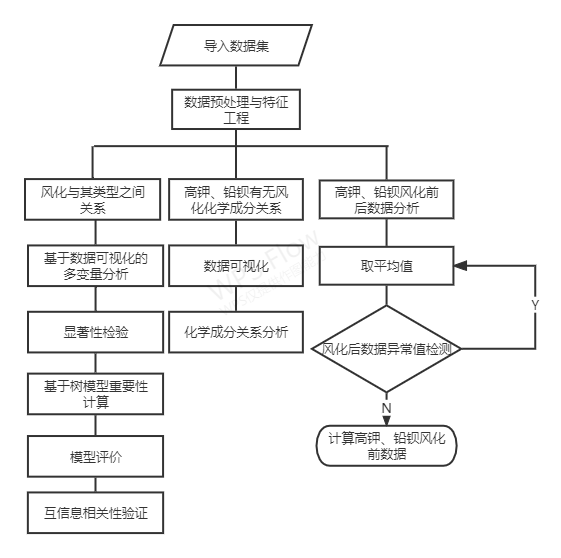
\includegraphics[width=0.95\textwidth]{1.png} 
	\caption{术中是否出现不良反应数据可视化图} 
	\label{Fig.main1} 
\end{figure}

分析图1中的术中是否出现三类不良反应的直方图,可以发现从数量上B药出现呛咳、体动、术中其他不良反应的数量比R药少,尤其是体动方面的不良反应在直观上两要差异最大,其他两种不良反应中B药几乎不出现不良反应,可以看到术中使用新药容易出现不良反应。

接下来利用和以上一样的方式对于手术后 24 小 时的不良的反应(恶心呕吐、嗜睡乏力、头昏头晕头痛、腹胀腹痛、其他不舒服) 的数 据做出数据可视化图来进一步分析新药组和原有药组之间是否存在差异, 得到数据可视化图如下所示:

\begin{figure}[H] % 这个H不要动!
	\centering % 不要动!
	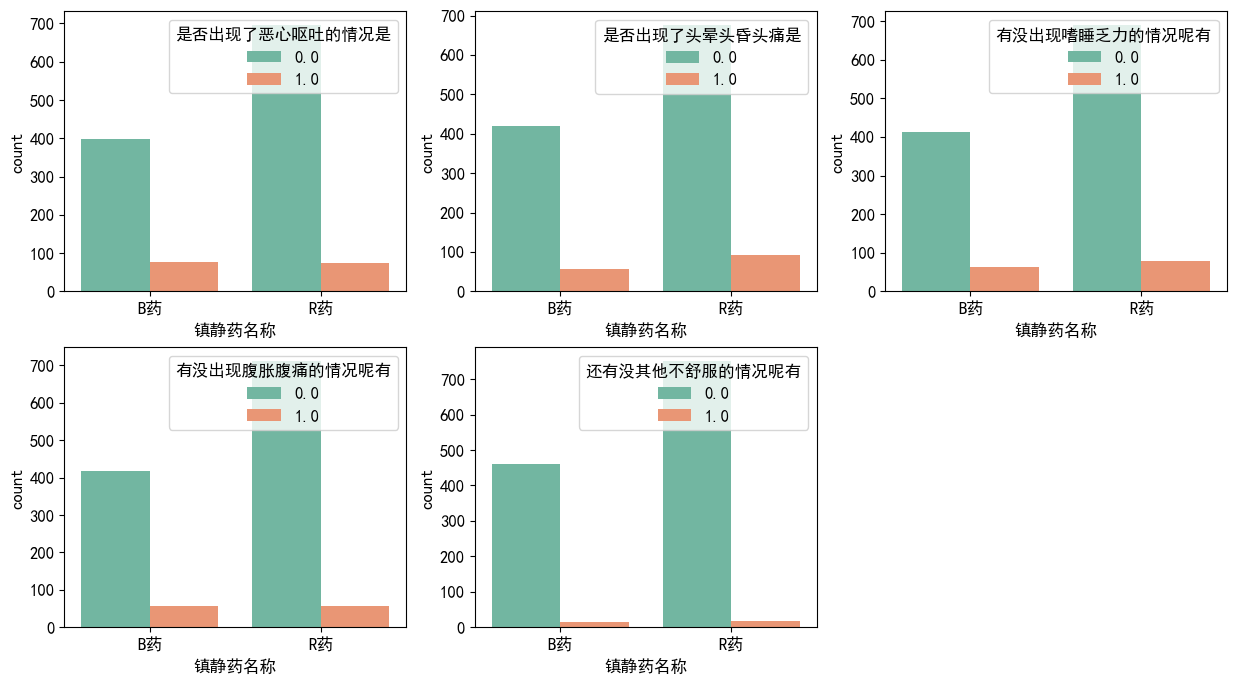
\includegraphics[width=0.95\textwidth]{2.png} 
	\caption{手术后是否出现不良反应数据可视化图} 
	\label{Fig.main2} 
\end{figure}

分析图2的术后是否出现三类不良反应的直方图,可以发现从数量上,B药出现恶心呕吐、嗜睡乏力、腹胀腹痛、其他不舒服的不良反应数量基本与R药持平,只有出现头晕头昏头痛的不良反应的数量上少于R药。从比例上看,R药的基数大于B药,但是出现恶心呕吐、嗜睡乏力、腹胀腹痛、其他不舒服的不良反应数量却与B药持平,可以出在术后使用R药不容易出现不良反应。


\subsubsection{基于卡方检验的定量差异探究}

接下来利用卡方检验分别对手术期间和手术24小时后的出现不良反应来定量探究两组药物之间是否具有显著差异,对于分类问题可以列出交叉表,发现总样本大于40且每个类别的理论频数大于5可用卡方检验:

\begin{enumerate}
    \item 原假设${{H}_{0}}$:两种药没有显著差异;
    \item 备择假设${{H}_{1}}$:两种药有显著差异;
\end{enumerate}

首先计算检验统计量:

\begin{equation}
    {{\chi }^{2}}=\sum\limits_{i=1}^{m}{\sum\limits_{j=1}^{k}{\frac{{{O}_{ij}}-{{E}_{ij}}}{{{E}_{ij}}}}}.
\end{equation}
接着计算自由度:

\begin{equation}
    df=\left( m-1 \right)\times \left( k-1 \right).
\end{equation}
利用卡方分布的累积分布计算值:

\begin{equation}
    p=1-F\left( {{\chi }^{2}},df \right).
\end{equation}
若检验统计量大于临界值(p值大于显著性水平0.05),不能拒绝原假设,两种药没有显著差异;若检验统计量小于临界值(p值小于显著性水平0.05),拒绝原假设,两种药有显著差异。

\begin{table}[H]
	\centering  % 不要动!
    \caption{卡方检验结果}
	\begin{tabular}{c c c c}  % 有几列就要有几个c,c与c之间用空格
		\toprule[1.5pt]  % 不要动!
		名称 & 卡方值 & p值 & 自由度  \\   % 列与列之间用  & 隔开,下同
		\midrule[1pt]    % 不要动!
        呛咳 & 	13.514691 & 0.000236 &	1  \\
        体动 & 	7.278738 & 	0.006977	 & 1  \\
        术中其他不良反应 & 	12.815257 &	0.000343 &	1  \\
        恶心呕吐 & 	11.929730 &	0.000552 &	1  \\
        嗜睡乏力 & 	0.003899 &	0.950210 &	1  \\
        头昏头晕头痛 & 	2.333728 &	0.126598 &	1  \\
        腹胀腹痛 & 	7.536825 &	0.006045 &	1  \\
        其他不舒服 & 	0.226608	 & 0.634050 &	1  \\
		\toprule[1.5pt]  % 不要动!
	\end{tabular}  
\end{table} 


由表可知,“咳嗽”、“体动”以及“术中其他反应”的卡方检验结果的p值均小于0.05,故认为在术中不良反应关于药物类别具有显著差异;“是否出现恶心呕吐”和“是否出现腹胀腹痛”的情况的卡方检验的结果p值小于0.05,两药物之间有显著差异;“是否出现头晕头昏头痛”、“是否有嗜睡乏力情况”、“是否有其他不舒服”情况的p值均大于0.05,故其关于药物类别无显著差异。


\subsection{基于KNN的不良反应预判}

\subsubsection{模型建立}

题目要求根据患者基本信息和镇静药物种类,对患者术中、术后 24h 的不良反应进行预判。首先先对手术期间和手术后是否产生不良反应进行数据可视化,得到结果如下图所示:

\begin{figure}[H] % 这个H不要动!
	\centering % 不要动!
	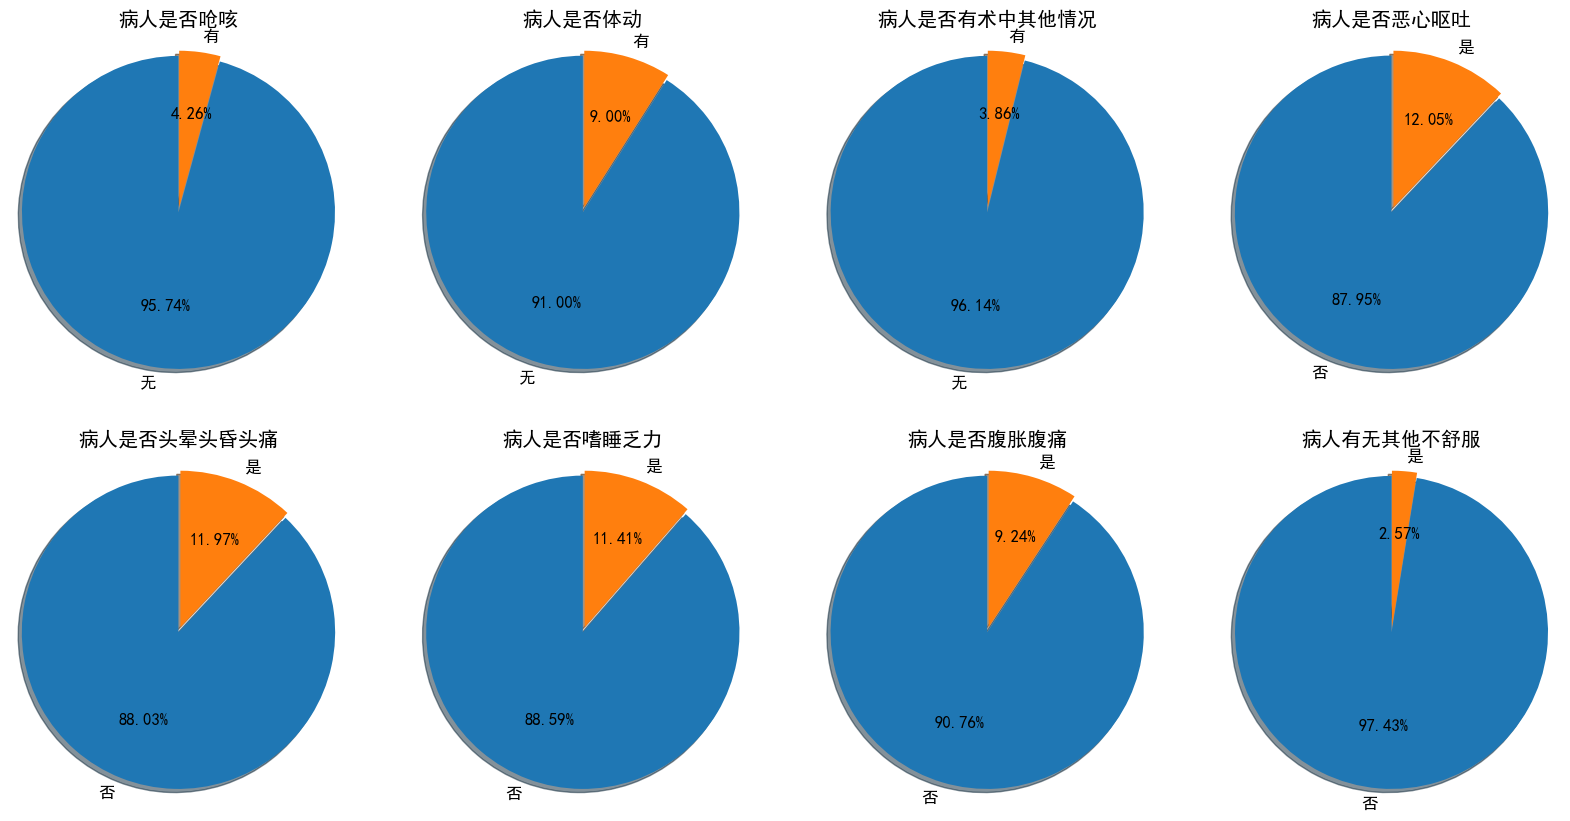
\includegraphics[width=0.95\textwidth]{3.png} 
	\caption{对不良反应的分布可视化} 
	\label{Fig.main3} 
\end{figure}

由上图可知,未出现呛咳、体动、术中其他、恶心呕吐、头晕头昏头痛、嗜睡乏力、腹胀腹痛、其他不舒服的的占比均超过87\%,即术中和术后未出现不良反应远远超过出现不良反应的数量,针对此类情况,对数据进行上采样。设各标签少数类样本数量为$k$,则有:

\begin{equation}
    P(x|y=1,D_{up}) = \dfrac{\sum_{i=1}^{k} [x_i=x]}{k}.
\end{equation}
其中$x_i$ 表示第 $i$ 个采样得到的少数类样本的特征。再将上采样后的数据集划分为训练集和测试集,建立KNN模型对训练集进行拟合,再使用测试集来评估模型的性能。

近邻法使用的模型主要有三个基本要素——距离度量, ${{L}_{3}}\left( {{\overrightarrow{x}}_{i}},{{\overrightarrow{x}}_{j}} \right)$值的选择和分类决策规则决定. 近邻法中,当训练集、距离度量、 ${{L}_{3}}\left( {{\overrightarrow{x}}_{i}},{{\overrightarrow{x}}_{j}} \right)$值及分类决策规则确定后,对于任何一个新的输入实例,它所属的类唯一地确定.这相当于根据上述要素将特征空间划分为一些子空间,确定子空间里每个点所属的类.

\begin{enumerate}
    \item \textbf{度量距离}
  
    本文使用的主要是闵可夫斯基(Minkowski)距离.原理如下:设特征空间$\chi$是$n$维实数向量空间${{R}^{n}},{{\overrightarrow{x}}_{i}},{{\overrightarrow{x}}_{j}}\in \chi .$
  
    \begin{equation}
        {{\overrightarrow{x}}_{i}}={{\left( x_{i}^{\left( 1 \right)},x_{i}^{\left( 2 \right)},\cdots ,x_{i}^{\left( n \right)} \right)}^{T}},{{\overrightarrow{x}}_{j}}={{\left( x_{j}^{\left( 1 \right)},x_{j}^{\left( 2 \right)},\cdots ,x_{j}^{\left( n\right)} \right)}^{T}},
    \end{equation}

    ${\overrightarrow{x}_{i}},{\overrightarrow{x}_{j}}$的距离定义为:

    \begin{equation}
        {{L}_{3}}\left( {{x}_{i}},{{x}_{j}} \right)={{\left( \sum\limits_{l=1}^{n}{{{\left| x_{i}^{\left( l \right)},x_{j}^{\left( l \right)} \right|}^{3}}} \right)}^{\frac{1}{3}}}.
    \end{equation}

    \item \textbf{$k$的取值}
    
    如果选择的$k$值较小,模型“学习”的近似误差就会减小,但“学习”的估计误差会增大.$k$值的减小就意味着整体模型变得复杂,容易发生过拟合.如果选择的$k$值较大,则相反,一般使用交叉验证确定$k$值。
    
    \item \textbf{分类决策规则}
    
    
    $k$近邻法中分类决策规则往往是多数表决,即由输入实例的$k$个邻近的训练实例中的多数类决定输入实例的类.
    分类函数为:
    
    \begin{equation}
        f:{{R}^{n}}\to \left\{ {{c}_{1}},{{c}_{2}},\cdots ,{{c}_{K}} \right\}.
    \end{equation}
    那么误分类的概率是:
    
    \begin{equation}
        P\left( Y\ne f\left( X \right) \right)=1-P\left( Y\equiv f\left( X \right) \right).
    \end{equation}
    对给定的实例$\overrightarrow{x}\in \chi$,其最近邻的$k$个训练实例点构成的集合${{N}_{k}}\left( \overrightarrow{x} \right)$。如果涵盖${{N}_{k}}\left( x \right)$的区域的类别是${{c}_{j}}$,那么误分类概率是:
    
    \begin{equation}
        \frac{1}{k}\sum\limits_{{{\overrightarrow{x}}_{i}}\in {{N}_{k}}\left( \overrightarrow{x} \right)}{I\left( {{y}_{i}}\ne {{c}_{j}} \right)}=1-\frac{1}{k}\sum\limits_{{{\overrightarrow{x}}_{i}}\in {{N}_{k}}\left( \overrightarrow{x} \right)}{I\left( {{y}_{i}}={{c}_{j}} \right)}.
    \end{equation}
    要使误分类率最小即经验风险最小,就要使$\sum\limits_{{{\overrightarrow{x}}_{i}}\in {{N}_{k}}\left( \overrightarrow{x} \right)}{I\left( {{y}_{i}}={{c}_{j}} \right)}$最大,所以多数表决规则等价于经验风险最小化。 
    
    \item \textbf{KNN的实现—kd树}
    
    更优化处理一般使用kd树。为了更高效地找到k个近邻样本,使用k-d树来组织训练数据集。kd树是一种二叉树结构,每个节点代表一个训练样本。通过对训练样本递归地划分空间,可以构建出一棵kd树。在查询测试样本的k个近邻时,可以通过遍历k-d树来快速找到距离测试样本最近的k个训练样本。
    
    因此,k-d树可以被看作是k近邻法模型中实现近邻搜索的数据结构,它可以大大提高模型的预测效率。为了进一步提高模型的准确率,使基于GridSearchCV实现带交叉验证的网格搜索对KNN模型进行超参数优化。参数选择与最终结果为:
    
    \begin{table}[H]
        \centering  
        \caption{GridSearchCV对KNN模型调参结果}
        \begin{tabular}{c c c}  
        	\toprule[1.5pt]  
        	参数 & 取值范围 & 最优结果 \\  
        	\midrule[1pt]    
        	algorithm & [auto, ball\_tree, kd\_tree, brute] & auto\\ 
        	leaf\_size & np.arange(10,51,10) & 10 \\
        	weights & [uniform, distance] & uniform \\
        	n\_neighbors & np.arange(1,11,1) & 1 \\
        	p & [1,2,3] & 3 \\ 
        	\toprule[1.5pt]  
        \end{tabular}  
    \end{table} 
\end{enumerate}

\subsubsection{模型求解}


基于Scikit-Learn库按上文最有参数初始化模型,分别以“呛咳”、“体动”、“术中其他不良反应”、“恶心呕吐”、“嗜睡乏力”、“头昏头晕头痛”、“腹胀腹痛”、“术后其他不舒服”八个为标签生成数据集,按4:1的比例划分数据集,并使用训练集对初始化的KNN模型进行训练。使用KNN模型对测试集的特征空间进行预测,并使用分类器常见评价指标进行评价,以此来判断此模型是否可以用来根据患者基本信息和镇静药物种类,对患者术中、术后 24小时的不良反应进行预判,得到结果如下表:

\begin{table}[H]
    \centering  
    \caption{KNN测试结果评价}
    \begin{tabular}{c c c c c c}  
    	\toprule[1.5pt]  
    	标签名称 & 测试选项 & 准确率 & 召回率 & F1分数 & 支持率 \\  
    	\midrule[1pt]    
    	\multirow{2}{*}{呛咳} & 无 & 1.00	& 0.93	& 0.96	& 247 \\ 
    	                      & 有 & 0.93	& 1.00	& 0.96	& 230 \\
    	\multirow{2}{*}{体动} & 无 & 1.00	& 0.92	& 0.96	& 224 \\
    	                      & 有 & 0.93	& 1.00	& 0.96	& 228 \\
    	\multirow{2}{*}{术中其他不良反应} & 无 & 1.00   & 0.96  & 0.98  & 250 \\ 
    	                                  & 有 & 0.93	& 1.00	& 0.96	& 230 \\
    	\multirow{2}{*}{恶心呕吐} & 无 & 0.98 & 0.88 & 0.93 & 228 \\
    	                          & 有 & 0.88 & 0.98 & 0.93 & 210 \\
    	\multirow{2}{*}{嗜睡乏力} & 无 & 0.99 & 0.86 & 0.92 & 232 \\ 
    	                          & 有 & 0.86 & 0.99 & 0.92 & 207 \\
    	\multirow{2}{*}{头昏头晕头痛} & 无 &  1.00 & 0.87 & 0.93 & 221 \\
    	                              & 有 &  0.88 & 1.00 & 0.94 & 221 \\
    	\multirow{2}{*}{腹胀腹痛} & 无 &  1.00 & 0.92 & 0.96 & 224 \\ 
    	                          & 有 &  0.93 & 1.00 & 0.96 & 228 \\
        \multirow{2}{*}{术后其他不舒服} & 无 & 1.00 & 0.97 & 0.99 & 245 \\
    	                      & 有 & 0.97  & 1.00  & 0.99  & 241  \\ 
    	\toprule[1.5pt]  
    \end{tabular}  
\end{table} 

为了让结果更直观,本文基于Scikit-Learn将测试结果利用混淆矩阵和ROC图可视化,并计算出KNN在测试集上预测的AUC值,以“术后有无其他不舒服”为例的可视化结果如下所示:

\begin{figure}[H] % 这个H不要动!
	\centering % 不要动!
	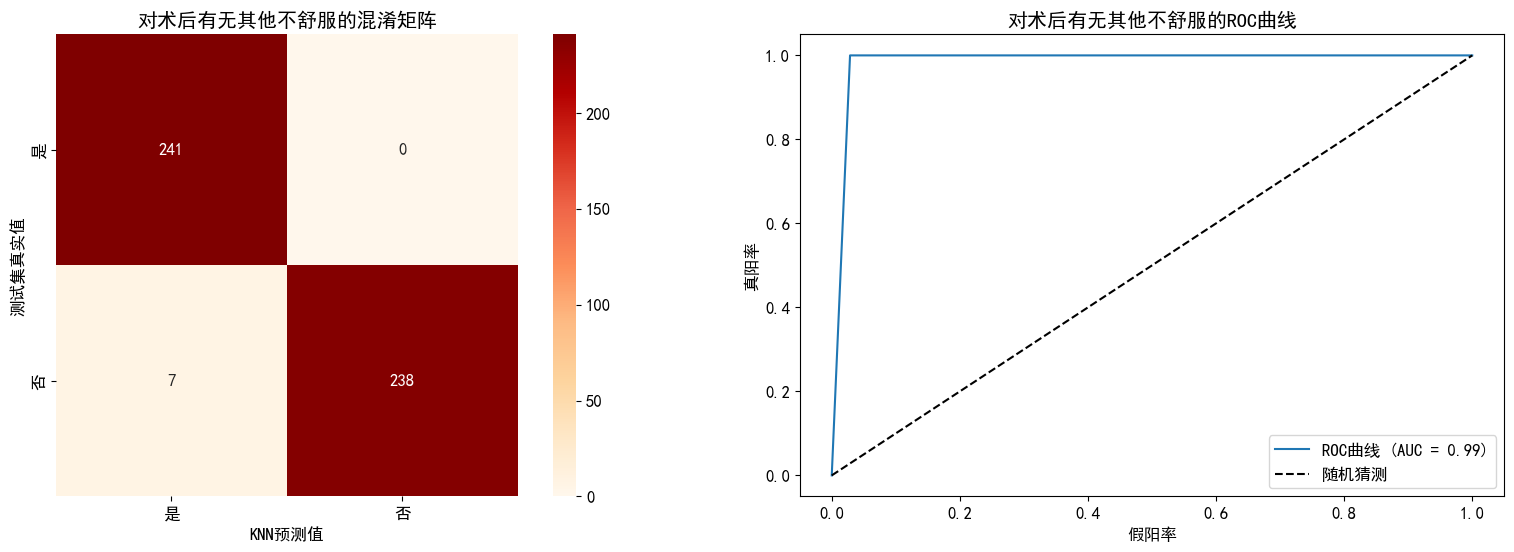
\includegraphics[width=0.95\textwidth]{4.png} 
	\caption{术后有无其他不舒服热力图和ROC曲线} 
	\label{Fig.main4} 
\end{figure}

由上图可以看到对角线上的数字相对较大,说明模型的分类效果比较好,但是对于“否”类别的预测效果略微不如“是”类别。另外,热力图的颜色也提供了直观的参考,颜色越深表示数量越多,可以看到"是"类别的预测结果相对比较准确,因此相应的颜色也比较深;ROC曲线看真阳率高,综上所述,KNN模型性能良好。完整的KNN测试结果的混淆矩阵、ROC图详见附录A。基于测试结果的评价,本文认为此模型可用来预判术中和术后24小时的不良反应出现情况。





















































































